\documentclass[10pt,a4paper,titlepage,oneside]{article}
\usepackage{LabProtocol}

\exercise{Exercise I}

% enter your data here
\authors{
	Vorname Nachname, Matr. Nr. 0123456 \par
	{\small e0123456@student.tuwien.ac.at} \par
}


\begin{document}

\maketitle


%████████╗ █████╗ ███████╗██╗  ██╗     ██╗
%╚══██╔══╝██╔══██╗██╔════╝██║ ██╔╝    ███║
%   ██║   ███████║███████╗█████╔╝     ╚██║
%   ██║   ██╔══██║╚════██║██╔═██╗      ██║
%   ██║   ██║  ██║███████║██║  ██╗     ██║
%   ╚═╝   ╚═╝  ╚═╝╚══════╝╚═╝  ╚═╝     ╚═╝
\Task{Introduction and Preparations}

\begin{qa}{Create a screenshot of the RTL netlist viewer, showing how the outputs of the PLL are connected to the rest of the system!}
	\begin{figure}[h!]
		\centering
		% \includegraphics[width=1.0\linewidth]{your filename here}
		\dummyimage
		\caption{RTL netlist viewer screenshot}
	\end{figure}
\end{qa}
%%%%%%%%%%%%%%%%%%%%%%%%%%%%%%%%%%%%%%%%%%%%%%%%%%%%%%%%%%%%%%%%%%%%%%%%%%%%%%%%


%████████╗ █████╗ ███████╗██╗  ██╗    ██████╗ 
%╚══██╔══╝██╔══██╗██╔════╝██║ ██╔╝    ╚════██╗
%   ██║   ███████║███████╗█████╔╝      █████╔╝
%   ██║   ██╔══██║╚════██║██╔═██╗     ██╔═══╝ 
%   ██║   ██║  ██║███████║██║  ██╗    ███████╗
%   ╚═╝   ╚═╝  ╚═╝╚══════╝╚═╝  ╚═╝    ╚══════╝
\Task{GameCube Controller}

\begin{qa}{Analyse the resource usage of your \textsf{gc\_cntrl}! You can find this information in the compilation report under the entry ``Analysis\&Synthesis''. }
\centering
\begin{tabular}{l|ll}
	\hline
		                   & Combinational ALUTs & Dedicated Logic Registers  \\ \hline\hline 
	Absolute number            &                     &                            \\
	\% of whole design         &                     &                            \\
	\% of whole FPGA resources &                     &                            \\ \hline
\end{tabular}
\end{qa}

%%%%%%%%%%%%%%%%%%%%%%%%%%%%%%%%%%%%%%%%%%%%%%%%%%%%%%%%%%%%%%%%%%%%%%%%%%%%%%%%

%████████╗ █████╗ ███████╗██╗  ██╗    ██████╗ 
%╚══██╔══╝██╔══██╗██╔════╝██║ ██╔╝    ╚════██╗
%   ██║   ███████║███████╗█████╔╝      █████╔╝
%   ██║   ██╔══██║╚════██║██╔═██╗      ╚═══██╗
%   ██║   ██║  ██║███████║██║  ██╗    ██████╔╝
%   ╚═╝   ╚═╝  ╚═╝╚══════╝╚═╝  ╚═╝    ╚═════╝ 
\Task{Decimal Printer}

\begin{qa}{Include the state graph of the state machine you designed and briefly explain how it works.}

You can use \texttt{dia} to draw the diagram. The provided makefile automatically converts dia files to PDFs and places them in the \texttt{dia/pdf} directory.
However, any other method for drawing pictures is also fine. 

\begin{figure}[h!]
	\centering
	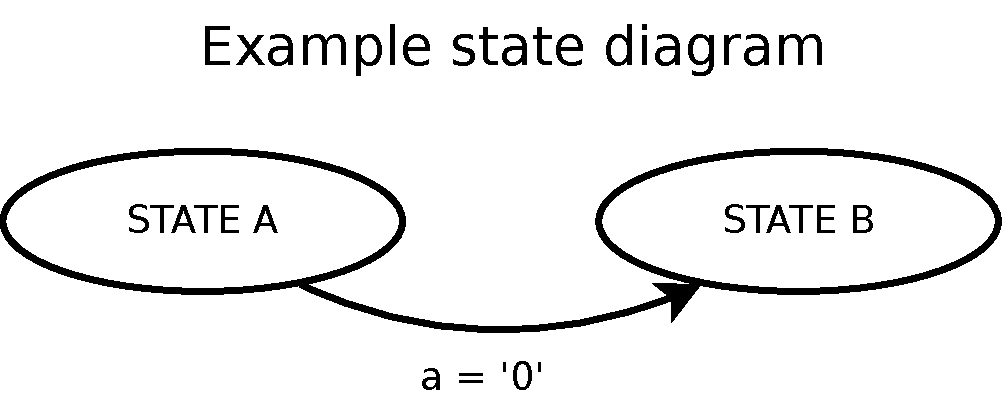
\includegraphics[width=0.75\linewidth]{dia/pdf/example_fsm.pdf}
	\caption{FSM state graph}
\end{figure}

\end{qa}

\end{document}
